Linking items and in general finding similarity among these already area-specific texts proved to be a problematic task. To test my algorithm I've decided to compare 89 SO questions with its matching Git issue and 4x one random git issue of the project. Results are plotted in figure \ref{fig:MatchesVsRandom}.\\

\begin{figure}[H]%
    \centering
	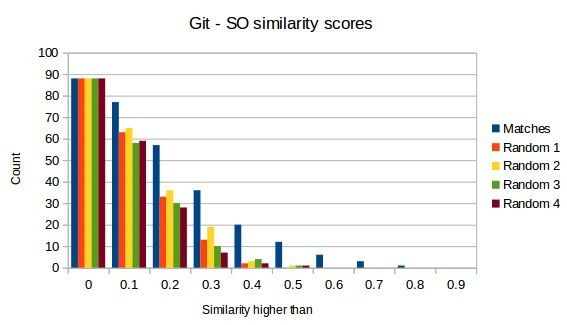
\includegraphics[width=15cm]{MatchesVsRandom.jpg}
    \caption{Similarity distribution of 89 matches and four data series of 89 random pairs}%
    \label{fig:MatchesVsRandom}%
\end{figure}

Results very clearly show that there is a particular similarity score, which is very hard to pass for two unrelated items. This score is obviously not constant and it depends on implementation of the similarity calculation. For my NLTK BoW algorithm used in figure \ref{fig:MatchesVsRandom}, the threshold is 0.4 or 0.5. Choosing the value of threshold would also depend on the  desired characteristics of a classifier and the prioritized metric. For example if a precision would be more important than recall, the ideal threshold would be 0.7 as it's the value which has never been passed by any of 356 non-matching pairs. The detailed table with the values for a figure \ref{fig:MatchesVsRandom} can be seen in appendix.\\
\\
I've executed the same steps using the Tf-Idf approach and although the values are different (as expected), they follow the same pattern. Figure \ref{fig:MatchesVsRandom_TfIdf} demonstrates these results and detailed values can again be found in appendix.

\begin{figure}[H]%
    \centering
	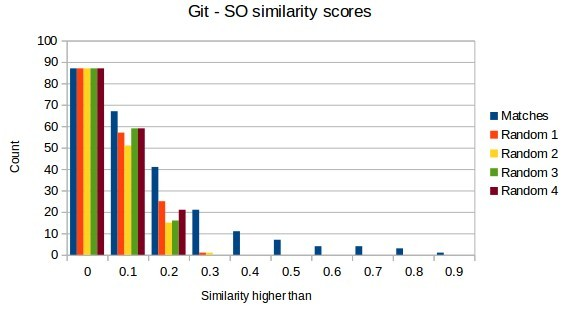
\includegraphics[width=15cm]{MatchesVsRandom_TfIdf.jpg}
    \caption{Similarity distribution of 89 matches and four data series of 89 random pairs}%
    \label{fig:MatchesVsRandom_TfIdf}%
\end{figure}

Despite clearly seeing possible threshold values, an algorithm which would label all the pairs above this threshold as matches would achieve very bad recall around 30\%. On the other side, precision would be 100\%. The potential problem is that the real-world ratio between matching and non-matching pairs rises exponentially with every new item on any side (Git issue, SO question). Testing the algorithm on bigger amount of data in the future could answer the question whether the threshold around 0.3 really proves as a unbreakable resistance for unrelated Git-SO pairs.\\
\\
Although I wasn't successful to such extent that the output are Git-StackOverflow or Git-Reddit True Positive pairs, I've pointed out some interesting results and data relationships.

\subsection{Stack Overflow}
The average similarity (using NLTK approach) between SO questions talking about particular issue and that particular issue description is 0.316 without body preprocessing and 0.292 with body preprocessing.

The distribution of similarities in buckets by increased by 0.05 can be seen in histogram in Figure \ref{fig:GitStackMatchesHistogram}

\begin{figure}[H]%
    \centering
	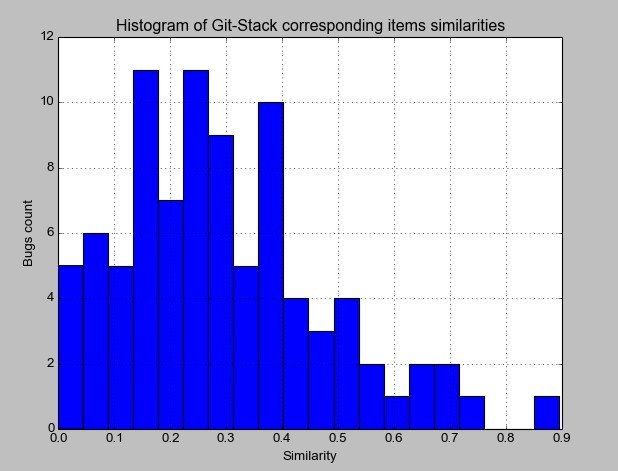
\includegraphics[width=8cm]{gitStackMatchesHistogram.jpg}
    \caption{Histogram of similarities distribution among git issues and their matching SO questions}%
    \label{fig:GitStackMatchesHistogram}%
\end{figure}

For random SO questions, amount of comparisons to Git issues needed to be limited. If every SO question would be compared to every Git issue, time of computation would exceed timeframe of this thesis. Every SO question was therefore compared to 20 random Git issues and resulting average similarity scores are in following figures.

\begin{figure}[H]%
    \centering
	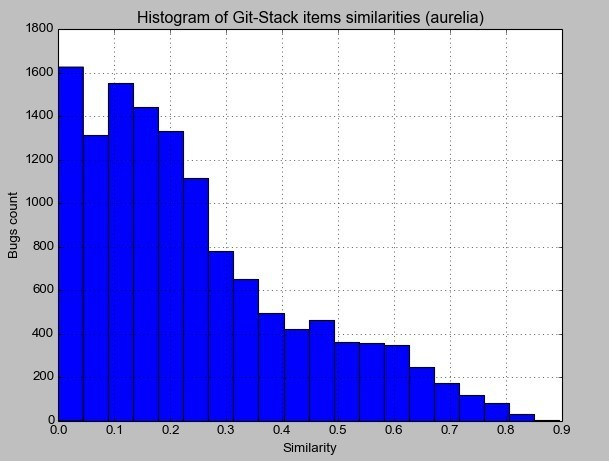
\includegraphics[width=8cm]{AureliaStackWithRandom20Bugs.jpg}
    \caption{Histogram of Aurelia SO questions and random git issues. Average similarity was 0.244}%
    \label{fig:AureliaStackWithRandom3Bugs}%
\end{figure}

\begin{figure}[H]%
    \centering
    \subfloat[EmberJS average similarity - 0.247]{{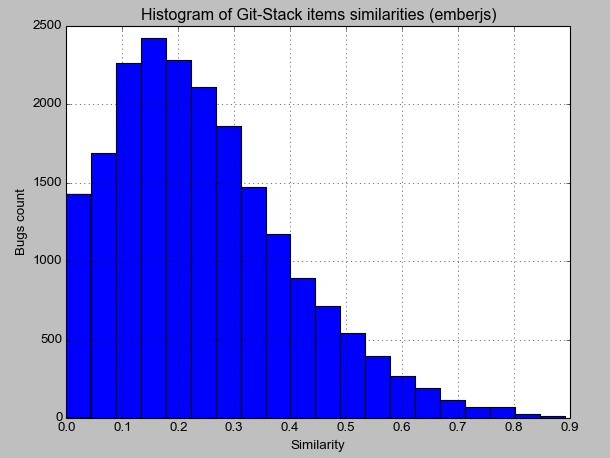
\includegraphics[width=6cm]{EmberStackWithRandom20Bugs.jpg} }}%
    \qquad
    \subfloat[Bower average similarity - 0.217]{{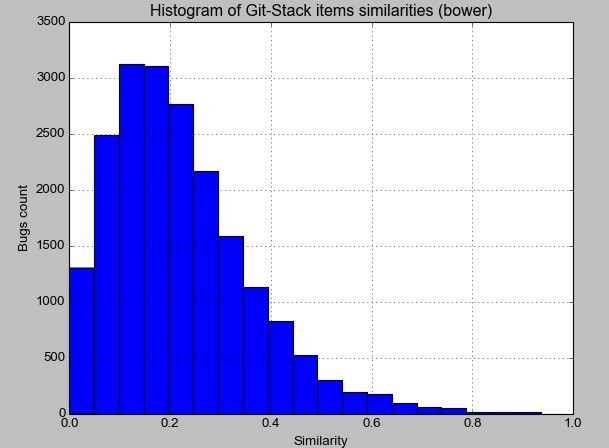
\includegraphics[width=6cm]{BowerStackWithRandom20Bugs.jpg} }}%
    \caption{EmberJS and Bower similarity histogram}%
    \label{fig:BowerEmberWithRandom3Bugs}%
\end{figure}

\begin{figure}[H]%
    \centering
    \subfloat[VueJS average similarity - 0.255]{{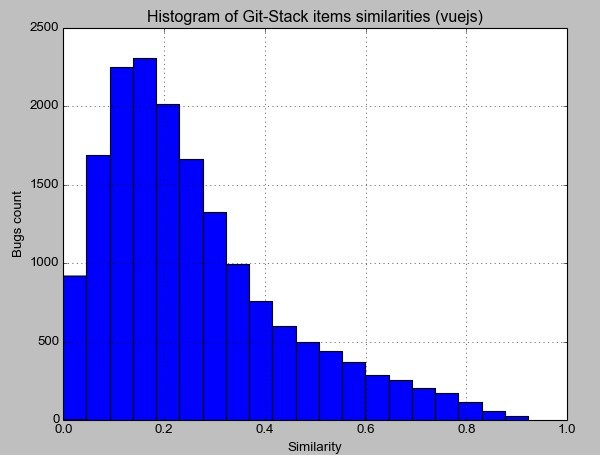
\includegraphics[width=6cm]{VueJSStackWithRandom20Bugs.jpg} }}%
    \qquad
    \subfloat[AngularJS average similarity - 0.258]{{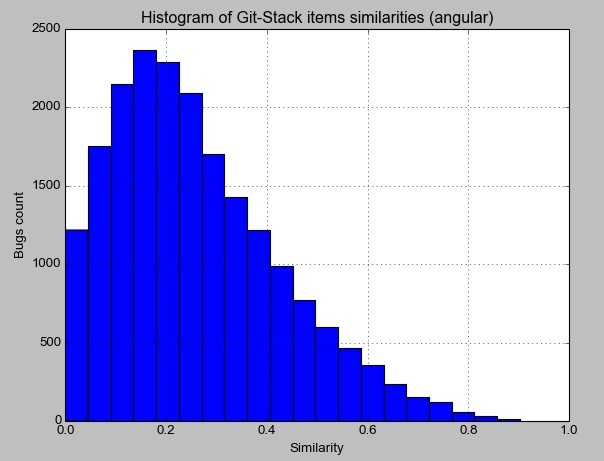
\includegraphics[width=6cm]{AngularStackWithRandom20Bugs.jpg} }}%
    \caption{VueJS and AngularJS similarity histogram}%
    \label{fig:VueAngularWithRandom3Bugs}%
\end{figure}


Table \ref{table:StackOverflowNLTKsimilarity} illustrates results of comparing Git bugs descriptions with SO questions talking about the same project issues and general issues. From values displayed, it's apparent that the difference between matches and random pairs is not very big. This is probably because all the texts about a particular project are already very specific and similar in their nature anyway.

\begin{table}[H]
\centering
\begin{tabular}{ |p{3cm}||p{4.5cm}|p{5.5cm}|}
 \hline
\textbf{ Framework }& \textbf{Own issues similarity}& \textbf{20 random issues similarity}\\
 \hline
 NodeJS   & 0.265 & 0.243\\ \hline
 AngularJS & 0.241 & 0.260\\ \hline
 EmberJS & 0.282 & 0.246\\ \hline 
 VueJS &   0.261 & 0.258\\ \hline
\end{tabular}
\caption{NLTK similarity values for SO questions}
\label{table:StackOverflowNLTKsimilarity}
\end{table}

\subsection{Reddit}Here I've calculated the similarity between the bug description and either particular comment in the reddit discussion which mentioned the bug or the whole discussion itself. Using NLTK BoW approach, average similarity score for all considered projects (NodeJS, AngularJS, VueJS and EmberJS) was 0.481 for the whole discussion and 0.368 for the comment itself. Scikit If-Idf values were 0.263 and 0.207 respectively. Detailed scores for each project can be found in table \ref{table:RedditNLTKsimilarity} for NLTK implementation and  table for \ref{table:RedditSCIKITsimilarity}. Subreddit for EmberJS didn't reference any of its own bugs.

\begin{table}[H]
\centering
\begin{tabular}{ |p{3cm}||p{3cm}|p{4cm}|}
 \hline
\textbf{ Framework }& \textbf{Bug comment}& \textbf{Whole discussion}\\
 \hline
 NodeJS   & 0.447 & 0.507\\ \hline 
 AngularJS & 0.306 & 0.57 \\ \hline 
 VueJS &   0.359 & 0.380\\ \hline
\end{tabular}
\caption{Reddit NLTK similarity values}
\label{table:RedditNLTKsimilarity}
\end{table}

\begin{table}[H]
\centering
\begin{tabular}{ |p{3cm}||p{3cm}|p{4cm}|}
 \hline
\textbf{ Framework }& \textbf{Bug comment}& \textbf{Whole discussion}\\
 \hline
 NodeJS   & 0.255 & 0.328\\ \hline 
 AngularJS & 0.168 & 0.278 \\ \hline 
 VueJS &  0.209  & 0.208\\ \hline
\end{tabular}
\caption{Reddit Scikit similarity values}
\label{table:RedditSCIKITsimilarity}
\end{table}

Both similarity calculations indicate that the semantic meaning of the bug is better expressed in the whole discussion rather than just the particular comment which referenced the bug. This made me question if it could be generalized that longer the text is, more similar it is to actual bug description. I've plotted a relationship between similarity score and length in Figures \ref{fig:SimilarityLengthRelationshipComment} and \ref{fig:SimilarityLengthRelationshipDiscussion}.

\begin{figure}[H]%
    \centering
	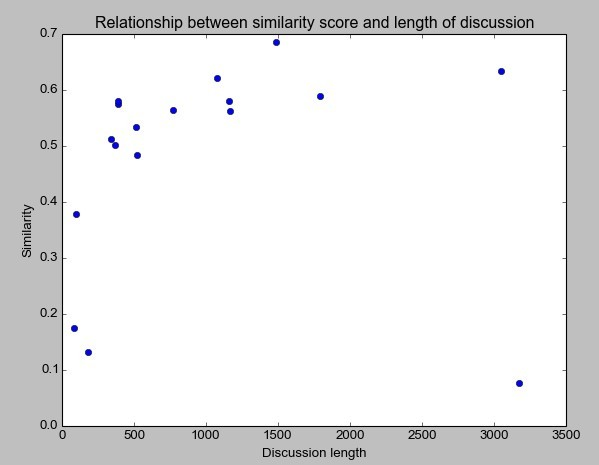
\includegraphics[width=8cm]{SimilarityLengthRelationshipDiscussion.jpg}
    \caption{Discussion lengths and similarity scores with the issue}%
    \label{fig:SimilarityLengthRelationshipDiscussion}%
\end{figure}

\begin{figure}[H]%
    \centering
	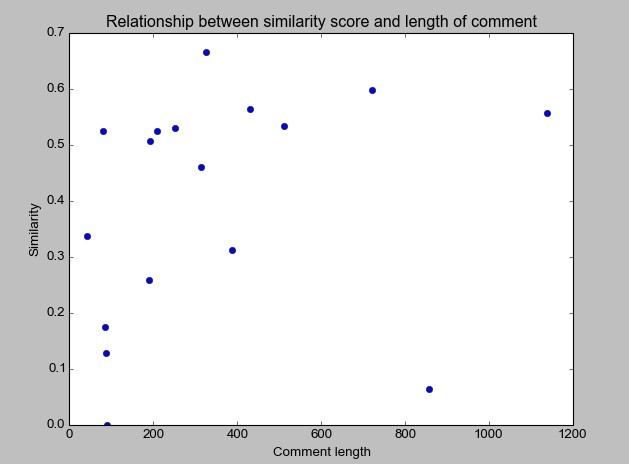
\includegraphics[width=8cm]{SimilarityLengthRelationshipComment.jpg}
    \caption{Comment lengths and similarity scores with the issue}%
    \label{fig:SimilarityLengthRelationshipComment}%
\end{figure}


